\documentclass[aspectratio=169]{beamer}

% ── Theme & colours ───────────────────────────────────────────────────────────
\usetheme{Madrid}
\usecolortheme{default}
\setbeamertemplate{navigation symbols}{}
\setbeamertemplate{footline}[frame number]

% ── Packages ──────────────────────────────────────────────────────────────────
\usepackage{graphicx}
\usepackage{booktabs}
\usepackage{amsmath}
\usepackage{algorithm}
\usepackage{algpseudocode}
\usepackage{xcolor}
\usepackage{tikz}
\usepackage{multirow}
% NOTE: do NOT load hyperref manually — beamer already loads it internally
\usepackage[style=numeric, sorting=none, backend=biber]{biblatex}
\addbibresource{references.bib}

% ── Custom colours ────────────────────────────────────────────────────────────
\definecolor{depotred}{RGB}{180,30,30}
\definecolor{gagreen}{RGB}{34,139,34}
\definecolor{impblue}{RGB}{30,90,180}

% ── Title info ────────────────────────────────────────────────────────────────
\title[CVRP -- Genetic Algorithm]{%
  Solving the Capacitated Vehicle Routing Problem\\
  with a Genetic Algorithm Metaheuristic}
\subtitle{CSE 462 -- Algorithm Engineering Course Project}
\author{Group 2 (Metaheuristic Sub-group)}
\institute{Department of Computer Science and Engineering}
\date{\today}

% =============================================================================
\begin{document}

\begin{frame}
  \titlepage
\end{frame}

% ── Outline ──────────────────────────────────────────────────────────────────
\begin{frame}{Outline}
  \tableofcontents
\end{frame}

% =============================================================================
\section{Problem Definition}
% =============================================================================

\begin{frame}{The Capacitated Vehicle Routing Problem (CVRP)}
  \begin{block}{Problem statement}
    Given a depot, a set of customers with known demands, a fleet of $k$
    identical vehicles each with capacity $C$, find a set of minimum-cost
    routes -- one per vehicle, all starting and ending at the depot -- such
    that every customer is visited exactly once and no route exceeds $C$.
  \end{block}

  \vspace{4pt}
  \begin{columns}
    \column{0.55\textwidth}
    \textbf{Formally:}
    \begin{itemize}
      \item Graph $G = (V, E)$,\; $V = \{0,1,\ldots,n\}$
      \item Node $0$ = depot;\; nodes $1\ldots n$ = customers
      \item Demand $d_i$ for customer $i$
      \item Distance $c_{ij}$ between nodes $i$ and $j$
      \item Minimize $\displaystyle\sum_{\text{routes}} \sum_{\text{edges}} c_{ij}$
      \item Subject to: capacity and single-visit constraints
    \end{itemize}

    \column{0.42\textwidth}
    \textbf{Complexity:}
    \begin{itemize}
      \item NP-hard (generalises TSP)
      \item Exact methods become intractable beyond $\approx$80 nodes
      \item Metaheuristics are the practical choice for real instances
    \end{itemize}
  \end{columns}
\end{frame}

\begin{frame}{Benchmark Datasets}
  Three standard TSPLIB-format benchmark sets are used throughout all
  experiments:
  \vspace{4pt}
  \begin{center}
  \begin{tabular}{lrrrl}
    \toprule
    Dataset & Instances & Nodes (range) & Capacity & Reference \\
    \midrule
    Augerat A  & 27 & 32--80   & 100       & \cite{augerat1995computational} \\
    Eilon E    & 13 & 13--101  & 200--6000 & \cite{christofides1979set}      \\
    Golden     & 20 & 200--483 & 550       & \cite{golden1998impact}         \\
    \bottomrule
  \end{tabular}
  \end{center}
  \vspace{4pt}
  \begin{itemize}
    \item Each instance comes with a \texttt{.vrp} definition file and
          a \texttt{.sol} file containing the known best solution and cost.
    \item Distances use the TSPLIB integer Euclidean convention:
          $d_{ij} = \lfloor \sqrt{(x_i-x_j)^2 + (y_i-y_j)^2} + 0.5 \rfloor$
    \item The Eilon E-n13 instance uses an explicit (LOWER\_ROW) distance matrix.
  \end{itemize}
\end{frame}

% =============================================================================
\section{Original Genetic Algorithm}
% =============================================================================

\begin{frame}{Genetic Algorithm -- Background}
  Genetic Algorithms (GAs) are population-based evolutionary search methods
  inspired by natural selection \cite{holland1975adaptation, goldberg1989genetic}.
  \vspace{6pt}

  \begin{columns}
    \column{0.5\textwidth}
    \textbf{Why GA for CVRP?}
    \begin{itemize}
      \item Can escape local optima via population diversity
      \item Flexible representation for combinatorial problems
      \item Easily extended with domain-specific operators
      \item No gradient information required
    \end{itemize}

    \column{0.48\textwidth}
    \textbf{Giant-tour representation}
    \begin{itemize}
      \item Chromosome = permutation of all $n$ customer IDs
      \item Decoded by greedy split: scan the tour and start a new route
            whenever the next customer would exceed $C$
      \item Simple, always feasible, no repair needed
    \end{itemize}
  \end{columns}
\end{frame}

\begin{frame}{Original GA -- Algorithm}
  \begin{algorithm}[H]
  \caption{Original Genetic Algorithm for CVRP}
  \begin{algorithmic}[1]
    \State $P \leftarrow$ \textbf{RandomPopulation}$(N_{\text{pop}})$
    \For{$g = 1$ \textbf{to} $G_{\max}$}
      \State Evaluate fitness: $f(c) = \text{TotalDist}(\text{Decode}(c))$ for all $c \in P$
      \State $P' \leftarrow$ \textbf{Elites}$(P,\, e)$  \Comment{keep top $e$ unchanged}
      \While{$|P'| < N_{\text{pop}}$}
        \State $p_1, p_2 \leftarrow$ \textbf{TournamentSelect}$(P,\, k=3)$
        \State $c_1, c_2 \leftarrow$ \textbf{OX1Crossover}$(p_1, p_2)$ with prob.\ $p_c$
        \State $c_1 \leftarrow$ \textbf{Mutate}$(c_1)$;\; $c_2 \leftarrow$ \textbf{Mutate}$(c_2)$
        \State Append $c_1, c_2$ to $P'$
      \EndWhile
      \State $P \leftarrow P'$
    \EndFor
    \State \Return best chromosome seen
  \end{algorithmic}
  \end{algorithm}
\end{frame}

\begin{frame}{Original GA -- Operators}
  \begin{columns}
    \column{0.48\textwidth}
    \textbf{Order Crossover (OX1)} \cite{davis1985applying}
    \begin{enumerate}
      \item Choose a random segment $[a, b]$ from parent $P_1$
      \item Copy $P_1[a\ldots b]$ into the child at positions $a\ldots b$
      \item Fill remaining positions from $P_2$ in order, wrapping around
    \end{enumerate}
    Preserves the relative ordering of customer visits.

    \vspace{8pt}
    \textbf{Mutation (50/50 choice)}
    \begin{itemize}
      \item \emph{Swap}: exchange two random positions
      \item \emph{Inversion}: reverse a random sub-segment
    \end{itemize}

    \column{0.48\textwidth}
    \textbf{Parameters used}
    \begin{center}
    \begin{tabular}{ll}
      \toprule
      Parameter & Value \\
      \midrule
      Population size     & 100  \\
      Generations         & 300  \\
      Crossover rate      & 0.9  \\
      Mutation rate       & 0.2  \\
      Tournament size     & 3    \\
      Elite size          & 5    \\
      Random seed         & 42   \\
      \bottomrule
    \end{tabular}
    \end{center}
  \end{columns}
\end{frame}

% =============================================================================
\section{Proposed Modifications (Improved GA)}
% =============================================================================

\begin{frame}{Proposed Modifications -- Overview}
  Three targeted improvements are proposed to address the main weaknesses
  of the original GA:

  \vspace{6pt}
  \begin{enumerate}
    \setlength{\itemsep}{8pt}
    \item \textbf{Nearest-Neighbour Seeded Initialisation}\\
          \textit{Problem solved}: random initialisation produces very poor
          starting tours; the GA wastes generations escaping terrible solutions.

    \item \textbf{Intra-route 2-opt Local Search}\\
          \textit{Problem solved}: crossover and mutation alone cannot reliably
          eliminate edge crossings inside a single route; local search is
          essential to reach high-quality routes.

    \item \textbf{Adaptive Mutation Rate}\\
          \textit{Problem solved}: a fixed mutation rate is either too low
          (population stagnates in a local optimum) or too high (good
          solutions are destroyed).
  \end{enumerate}
\end{frame}

\begin{frame}{Modification 1 -- Nearest-Neighbour Seeded Initialisation}
  \begin{block}{Idea}
    Seed 20\% of the initial population with greedy nearest-neighbour tours,
    each starting from a different customer.  The remaining 80\% stay random.
  \end{block}

  \vspace{4pt}
  \textbf{Nearest-neighbour heuristic}:
  \begin{enumerate}
    \item Start at a given customer
    \item Repeatedly move to the closest unvisited customer
    \item Stop when all customers are added
  \end{enumerate}

  \vspace{4pt}
  \textbf{Reasoning}:
  \begin{itemize}
    \item NN tours are typically 20--30\% above optimal, far better than random
    \item Provides the GA with diverse but high-quality starting seeds
    \item Retaining 80\% random individuals preserves population diversity
    \item Particularly impactful on large instances (Golden, 200--483 nodes)
          where random initialisation converges extremely slowly
  \end{itemize}
\end{frame}

\begin{frame}{Modification 2 -- Intra-route 2-opt Local Search}
  \begin{block}{Idea}
    Every $L$ generations, apply a 2-opt improvement pass to each route
    of every newly created offspring before inserting it into the population.
  \end{block}

  \vspace{4pt}
  \textbf{2-opt}: repeatedly reverse a sub-segment $[i,\,j]$ of a route if
  doing so reduces its travel distance \cite{lin1965computer}:
  \[
    \text{remove edges } (v_{i-1}, v_i)\text{ and }(v_j, v_{j+1});
    \quad\text{add } (v_{i-1}, v_j)\text{ and }(v_i, v_{j+1})
  \]

  \vspace{4pt}
  \textbf{Reasoning}:
  \begin{itemize}
    \item OX1 crossover preserves \emph{global} customer order but disrupts
          \emph{local} route geometry, creating crossings
    \item 2-opt directly eliminates these crossings within each route
    \item Applied periodically (every $L=10$ gen) -- not every generation --
          to bound the extra computation cost
    \item Routes longer than 40 nodes skip 2-opt to prevent $O(n^2)$ blow-up
  \end{itemize}
\end{frame}

\begin{frame}{Modification 3 -- Adaptive Mutation Rate}
  \begin{block}{Idea}
    Monitor stagnation (generations without improvement).  When stagnation
    exceeds a threshold, gradually raise the mutation rate to inject
    diversity.  Reset to the base rate upon finding a new best solution.
  \end{block}

  \vspace{4pt}
  \textbf{Rule}:
  \[
    \mu =
    \begin{cases}
      \mu_{\text{base}} & \text{if stagnation} < S_{\text{limit}} \\
      \min\!\Bigl(0.8,\;\mu_{\text{base}} \times
        \bigl(1 + \tfrac{\text{stagnation}}{S_{\text{limit}}}\bigr)\Bigr)
        & \text{otherwise}
    \end{cases}
  \]

  \textbf{Parameters}: $\mu_{\text{base}} = 0.2$,\; $S_{\text{limit}} = 25$.

  \vspace{4pt}
  \textbf{Reasoning}:
  \begin{itemize}
    \item A fixed low rate is insufficient to escape plateaus; a fixed high
          rate randomly destroys good building blocks
    \item Adaptive rate raises diversity only when the population is stuck,
          then returns to a conservative rate once improvement resumes
  \end{itemize}
\end{frame}

% =============================================================================
\section{Experimental Results}
% =============================================================================

\begin{frame}{Experimental Setup}
  \begin{columns}
    \column{0.5\textwidth}
    \textbf{GA Parameters}
    \begin{center}
    \begin{tabular}{ll}
      \toprule
      Parameter & Value \\
      \midrule
      Population size     & 100  \\
      Generations         & 300  \\
      Crossover rate      & 0.9  \\
      Base mutation rate  & 0.2  \\
      Tournament size     & 3    \\
      Elite size          & 5    \\
      2-opt interval $L$  & 10   \\
      Stagnation limit    & 25   \\
      Random seed         & 42   \\
      \bottomrule
    \end{tabular}
    \end{center}

    \column{0.48\textwidth}
    \textbf{Evaluation metric}
    \[
      \text{Gap\%} = \frac{\text{found} - \text{known best}}{\text{known best}} \times 100
    \]
    \begin{itemize}
      \item Lower gap = better solution
      \item Gap = 0\% means optimal solution found
      \item Both algorithms run from the same seed for fair comparison
      \item 60 instances total across 3 datasets
    \end{itemize}
  \end{columns}
\end{frame}

\begin{frame}{Results -- Dataset A (Augerat, 27 instances)}
  \begin{center}
  \small
  % FIX: tabular spec must match 6 data columns
  \begin{tabular}{lrrrrr}
    \toprule
    Instance & Optimal & Orig GA & Gap\% & Impr GA & Gap\% \\
    \midrule
    A-n32-k5  & 784  & 924  & 17.86 & 834  & 6.38 \\
    A-n33-k5  & 661  & 736  & 11.35 & 665  & 0.61 \\
    A-n38-k5  & 730  & 902  & 23.56 & 738  & 1.10 \\
    A-n45-k6  & 944  & 1292 & 36.86 & 1010 & 7.01 \\
    A-n53-k7  & 1010 & 1556 & 54.06 & 1093 & 8.22 \\
    A-n63-k10 & 1314 & 1841 & 40.11 & 1345 & 2.36 \\
    A-n80-k10 & 1763 & 2895 & 64.21 & 1933 & 9.64 \\
    \midrule
    \textbf{Avg (27)} & & & \textbf{+36.98} & & \textbf{+6.66} \\
    \bottomrule
  \end{tabular}
  \end{center}
\end{frame}

\begin{frame}{Results -- Dataset E (Eilon, 13 instances)}
  \begin{center}
  \small
  % FIX: tabular spec must match 6 data columns
  \begin{tabular}{lrrrrr}
    \toprule
    Instance & Optimal & Orig GA & Gap\% & Impr GA & Gap\% \\
    \midrule
    E-n13-k4   & 247  & 247  & 0.00   & 247  & 0.00  \\
    E-n23-k3   & 569  & 570  & 0.18   & 569  & 0.00  \\
    E-n30-k3   & 534  & 584  & 9.36   & 541  & 1.31  \\
    E-n51-k5   & 521  & 809  & 55.28  & 551  & 5.76  \\
    E-n76-k7   & 682  & 1213 & 77.86  & 786  & 15.25 \\
    E-n101-k8  & 815  & 1650 & 102.45 & 928  & 13.87 \\
    E-n101-k14 & 1067 & 1984 & 85.94  & 1256 & 17.71 \\
    \midrule
    \textbf{Avg (13)} & & & \textbf{+47.33} & & \textbf{+10.37} \\
    \bottomrule
  \end{tabular}
  \end{center}
\end{frame}

\begin{frame}{Results -- Dataset Golden (20 large instances)}
  \begin{center}
  \small
  % FIX: tabular spec must match 6 data columns
  \begin{tabular}{lrrrrr}
    \toprule
    Instance   & Optimal  & Orig GA & Gap\%  & Impr GA & Gap\%  \\
    \midrule
    Golden\_1  & 5623.47  & 22239   & 295.45 & 5809    & 3.30   \\
    Golden\_10 &  735.43  &  3443   & 368.17 &  752    & 2.25   \\
    Golden\_11 &  911.98  &  4847   & 431.47 &  908    & $-$0.44 \\
    Golden\_12 & 1100.67  &  6831   & 520.63 & 1118    & 1.57   \\
    Golden\_13 &  857.19  &  3054   & 256.31 &  955    & 11.41  \\
    Golden\_17 &  707.76  &  2323   & 228.24 &  822    & 16.14  \\
    Golden\_9  &  579.70  &  2228   & 284.35 &  554    & $-$4.43 \\
    \midrule
    \textbf{Avg (20)} & & & \textbf{+373.22} & & \textbf{+11.55} \\
    \bottomrule
  \end{tabular}
  \end{center}
  \vspace{2pt}
  \textit{\small Negative gaps: Improved GA found solutions better than the listed known best.}
\end{frame}

\begin{frame}{Summary of Results}
  \begin{center}
  \begin{tabular}{lrrrr}
    \toprule
    Dataset & \multicolumn{2}{c}{Avg Gap\% $\downarrow$} & \multicolumn{2}{c}{Avg Time (s)} \\
    \cmidrule(lr){2-3}\cmidrule(lr){4-5}
            & Original GA & Improved GA & Original GA & Improved GA \\
    \midrule
    A (27 inst.)      & +36.98 & +6.66  & $\sim$0.5  & $\sim$1.2  \\
    E (13 inst.)      & +47.33 & +10.37 & $\sim$0.8  & $\sim$4.0  \\
    Golden (20 inst.) & +373.22 & +11.55 & $\sim$3.0 & $\sim$98.0 \\
    \midrule
    \textbf{Overall (60)} & \textbf{+151.30} & \textbf{+9.09} & & \\
    \bottomrule
  \end{tabular}
  \end{center}
  \vspace{6pt}
  \begin{itemize}
    \item Improved GA is \textbf{16.6$\times$ closer to optimal} on average
    \item Largest gain on Golden (large instances): random init completely
          fails; NN + 2-opt brings gap from $>$370\% down to $\sim$11\%
    \item Small E instances (n $<$ 30): both algorithms find near-optimal
    \item Trade-off: Improved GA is $\sim$2.5$\times$ slower on average
  \end{itemize}
\end{frame}

\begin{frame}{Route Visualisation -- Example}
  \begin{columns}
    \column{0.49\textwidth}
    \textbf{Original GA} -- A-n32-k5 (cost = 924)
    \begin{center}
      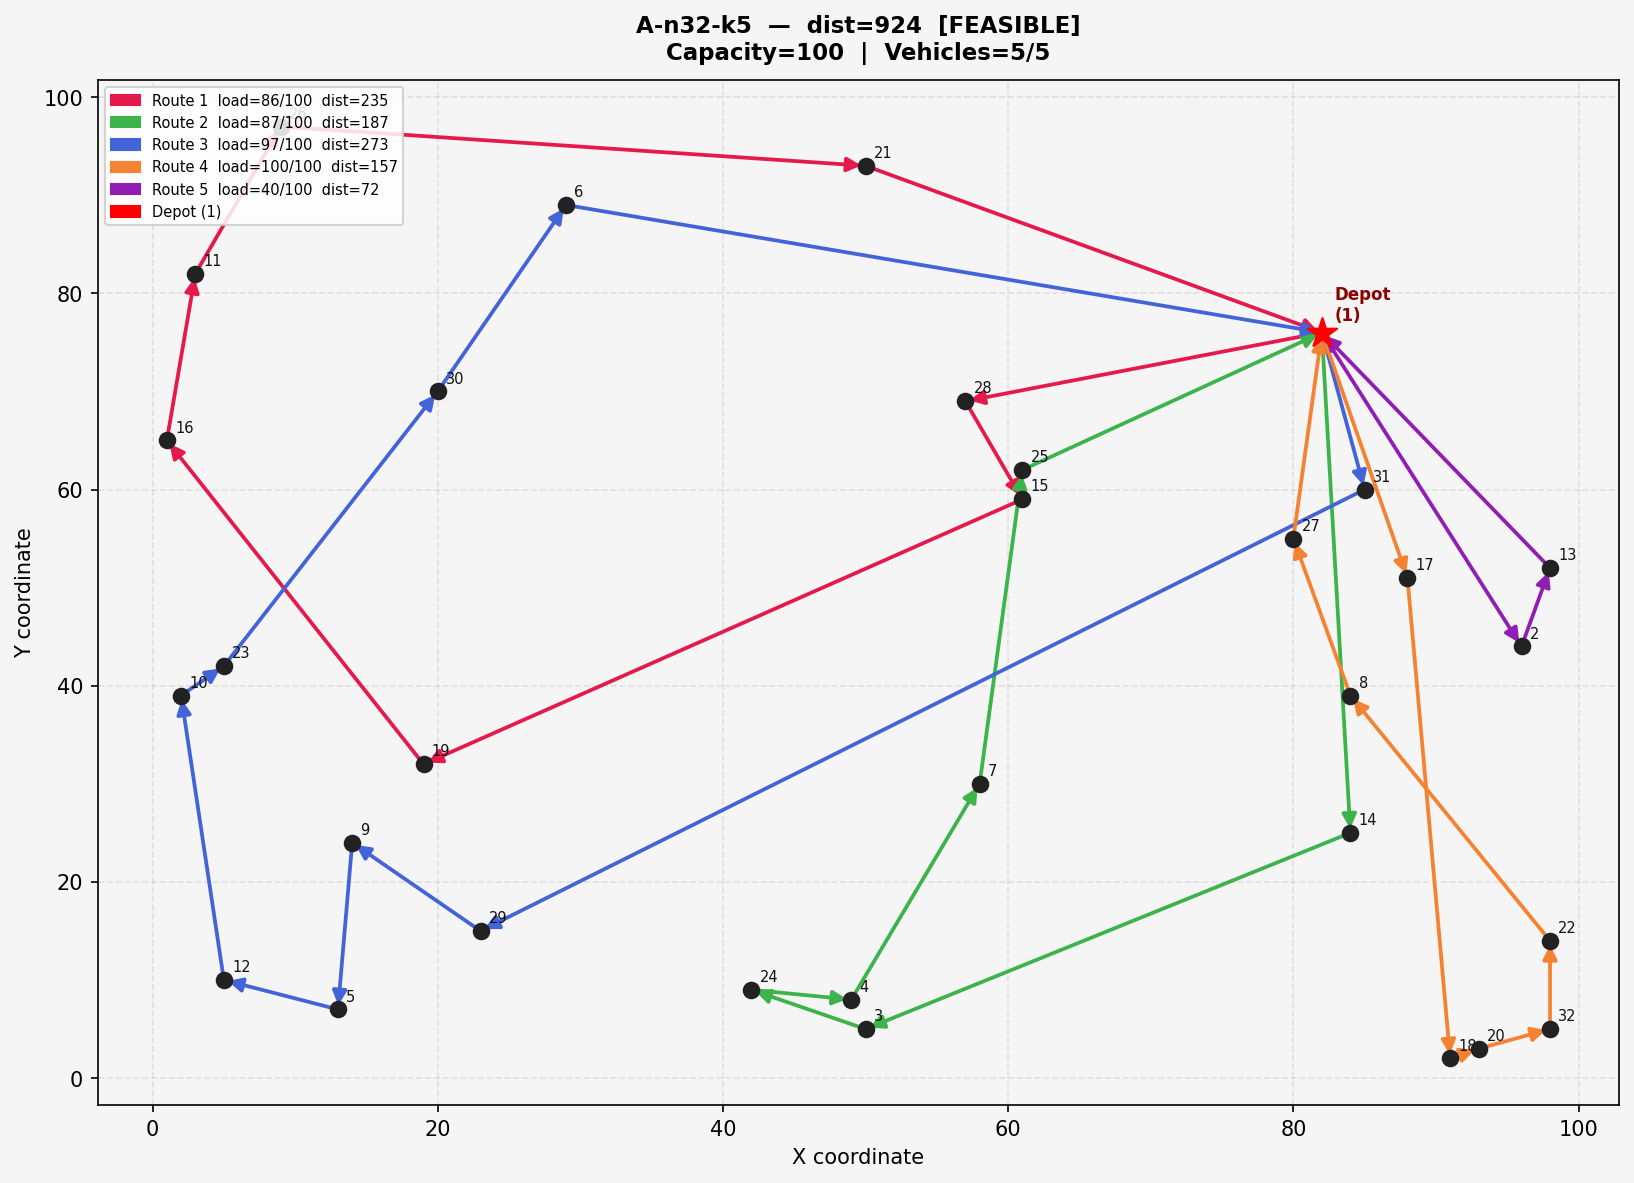
\includegraphics[width=\linewidth]{../metaheuristic/outputs/original_ga/A-n32-k5_plot.png}
    \end{center}

    \column{0.49\textwidth}
    \textbf{Improved GA} -- A-n32-k5 (cost = 834)
    \begin{center}
      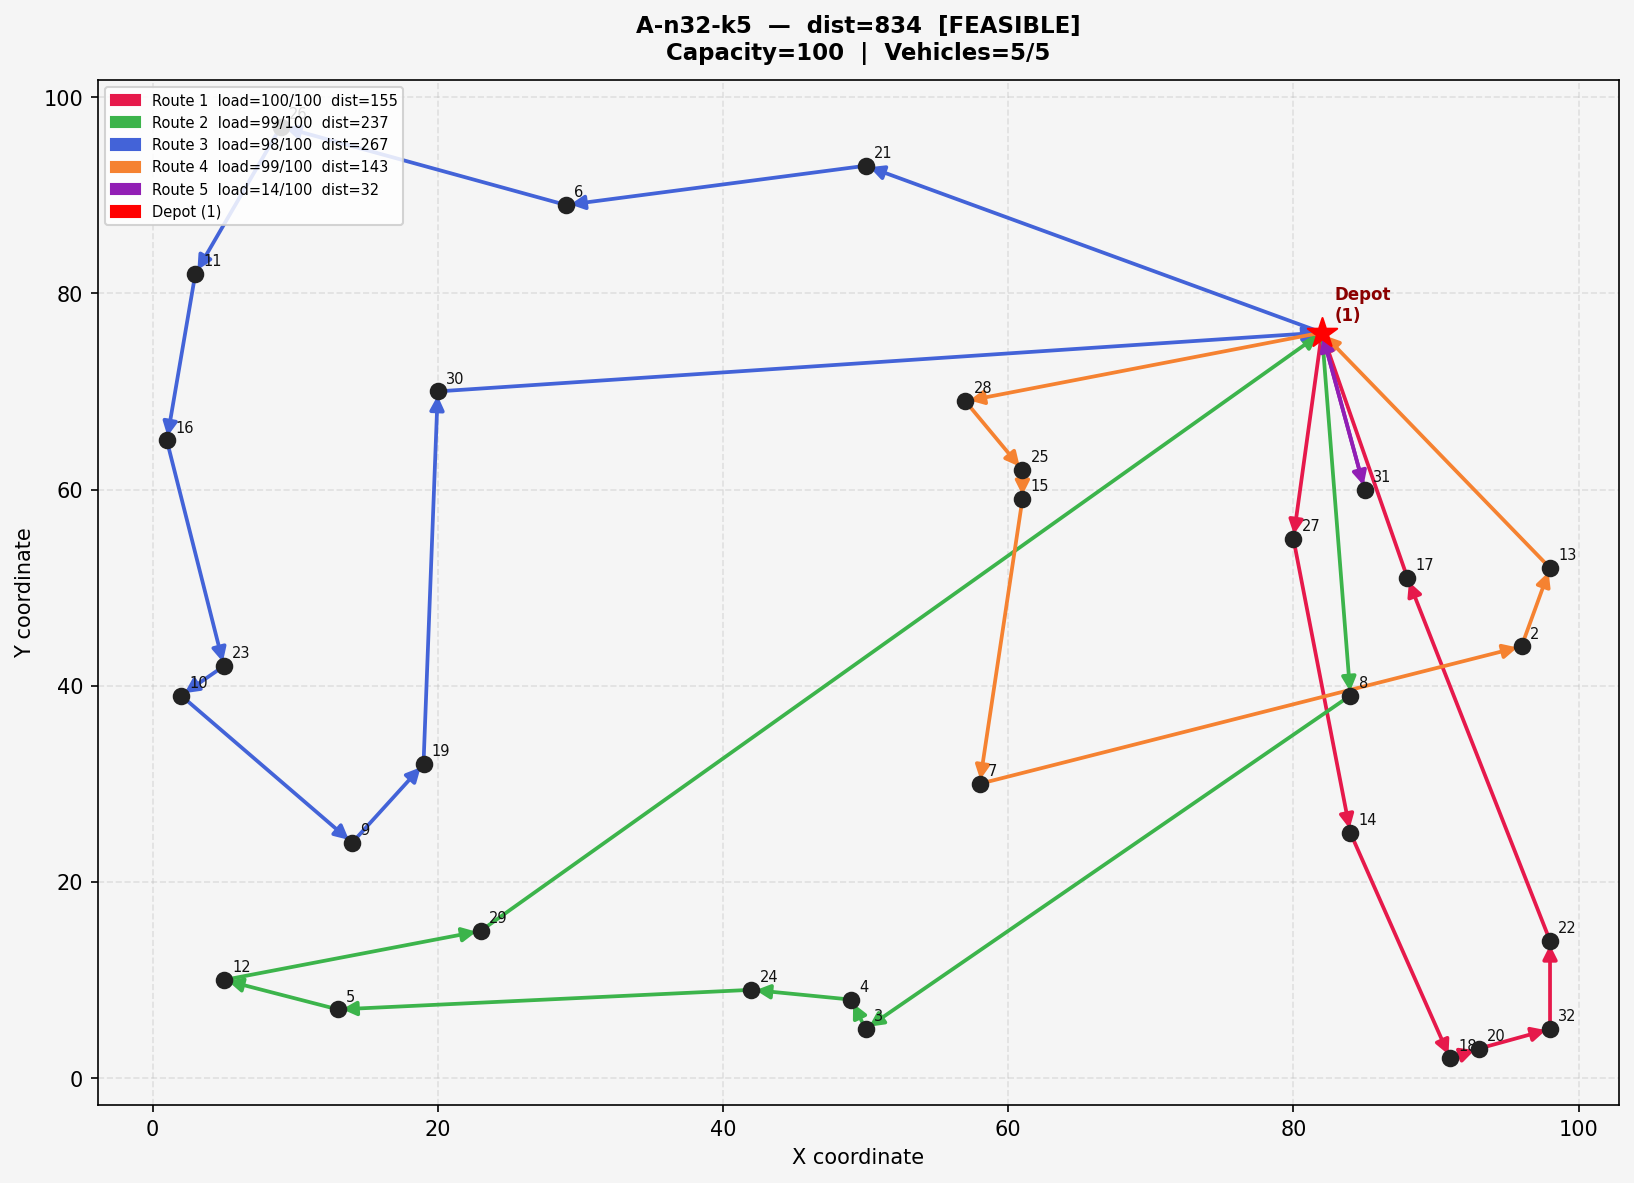
\includegraphics[width=\linewidth]{../metaheuristic/outputs/improved_ga/A-n32-k5_plot.png}
    \end{center}
  \end{columns}
  \vspace{4pt}
  \textit{Optimal = 784. Improved GA gap: 6.4\% vs Original GA gap: 17.9\%.
          The 2-opt local search visibly eliminates route crossings.}
\end{frame}

% =============================================================================
\section{Discussion \& Conclusion}
% =============================================================================

\begin{frame}{Discussion -- Impact of Each Modification}
  \begin{center}
  \begin{tabular}{lp{6.5cm}c}
    \toprule
    Modification & Main effect & Impact \\
    \midrule
    NN init       & Provides good starting tours; reduces wasted
                    early generations                              & High \\[4pt]
    2-opt LS      & Eliminates intra-route edge crossings that
                    genetic operators alone cannot remove          & Very high \\[4pt]
    Adaptive $\mu$ & Escapes stagnation without permanently
                    sacrificing exploitation quality               & Medium \\
    \bottomrule
  \end{tabular}
  \end{center}

  \vspace{6pt}
  \begin{itemize}
    \item The 2-opt local search is the most expensive modification but
          yields the greatest quality gain -- a classic metaheuristic trade-off
    \item NN initialisation is essentially free; its benefit is largest on
          the Golden benchmark where random tours are exponentially worse
    \item All three modifications work synergistically: NN provides a
          good starting point, 2-opt refines routes, and adaptive mutation
          explores further when the search plateaus
  \end{itemize}
\end{frame}

\begin{frame}{Conclusion}
  \begin{block}{Summary}
    We implemented and evaluated a standard Genetic Algorithm and an
    improved variant for the Capacitated Vehicle Routing Problem over
    60 benchmark instances from three well-known datasets.
  \end{block}

  \vspace{6pt}
  \textbf{Key findings:}
  \begin{itemize}
    \item The Original GA finds feasible solutions but struggles with solution
          quality, especially on large Golden instances ($>$370\% avg gap)
    \item All three proposed modifications contribute to quality improvement
    \item The Improved GA achieves an average gap of \textbf{9.09\%} vs
          \textbf{151.30\%} for the Original GA -- a 16.6$\times$ improvement
    \item The giant-tour + greedy split decoding always produces
          capacity-valid solutions with no repair step needed
  \end{itemize}

  \vspace{6pt}
  \textbf{Future work:}
  \begin{itemize}
    \item Or-opt and 3-opt moves for deeper local search
    \item Population restart strategies for very long runs
    \item Hybrid with exact solver for small sub-problems
  \end{itemize}
\end{frame}

% =============================================================================
\section*{References}
% =============================================================================

\begin{frame}[allowframebreaks]{References}
  \printbibliography[heading=none]
\end{frame}

\end{document}
